As a development method agile development was chosen for the project. But in order to maintain a good project management a tool for
agile development was needed. Git hub \cite{github} was the version control used and PivotalTracker \cite{pivotal}
was the agile tool of choice.

\begin{figure}[htp]
\centering
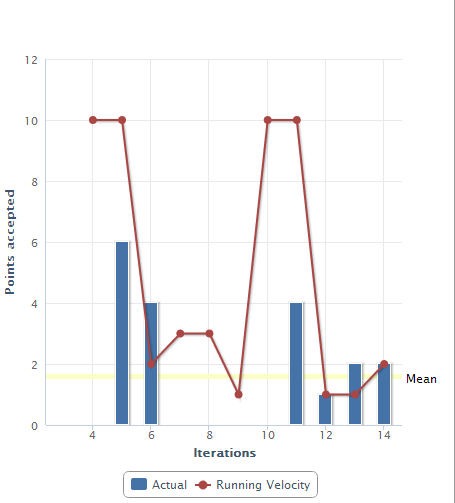
\includegraphics[scale=0.6]{Figures/pivotalGraph.png}
\caption{Velocity graph showing the sprints and the amount of work based on tickets completed in different iterations during first and second sprint}
\label{fig:pivotalGraph}
\end{figure}

PivotalTracker is a web based tool where all the development process was stored, place to put all the user stories, functional
and non-functional requirements, organize them and modify them easily. In the system it was easy to see when were the development bursts for the sprints and when was the post development time, when bugs were fixed, code was re-factored as seen in figure ~\ref{fig:pivotalGraph}.
This way the client can monitor how the actual development is going when was I working and on what feature. Pivotal tracker was used to monitor the progress
of the project as seen in figure ~\ref{fig:pivotalTracker}.

\begin{figure}[htp]
\centering
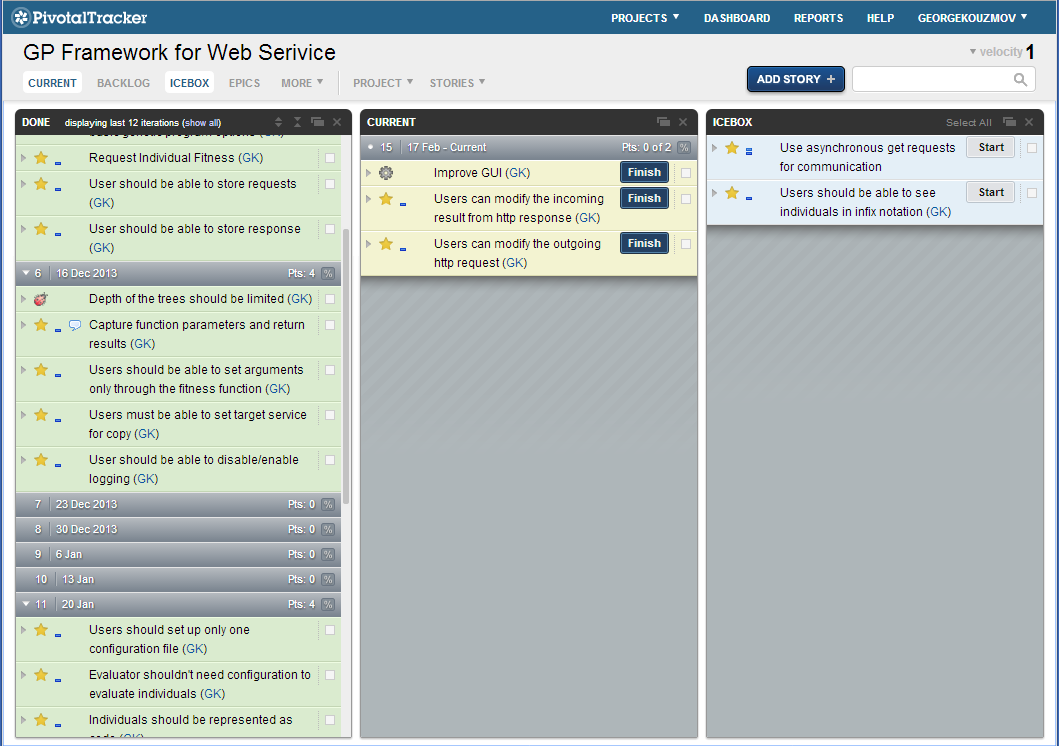
\includegraphics[scale=0.5]{Figures/pivotalTracker.png}
\caption{PivotalTracker and the way it is used by the project}
\label{fig:pivotalTracker}
\end{figure}

Git hub is the version control tool used for the project. Being a public code repository gave the opportunity to present the code easily to the client and
others as well. Frequent commits were done during the sprints. This way when the code broke during a sprint it could be reversed back to a working version.

